\section*{Experiment 2: To familiarize students with the operation of different electrical instruments including measuring equipments: Multi-meter, Frequency meter, Oscilloscope, Signal generator/Function generator}  
\addcontentsline{toc}{section}{Experiment 2: To familiarize students with the operation of different electrical instruments including measuring equipments: Multi-meter, Frequency meter, Oscilloscope, Signal generator/Function generator}


\subsection*{Summary}
This lab experiment will familiarize you with the operation of basic electrical instruments commonly used in electrical engineering and electronics. These instruments are essential for measuring various electrical quantities and analyzing electrical signals.

\subsection*{Learning Objectives}
\begin{enumerate}
    \item Identify and describe the functions of a multimeter, frequency meter, oscilloscope, and signal generator/function generator.
    \item Operate each instrument to measure voltage, current, resistance, frequency, and observe waveforms.
    \item Interpret the readings and waveforms displayed by each instrument.
\end{enumerate}

\subsection*{Equipment}
\begin{itemize}
    \item Multimeter (Digital or Analog)
    \item Frequency Meter
    \item Oscilloscope (Analog or Digital)
    \item Signal Generator/Function Generator
    \item Connecting leads (BNC cables for oscilloscope)
    \item Resistors (various values)
    \item Power supply (optional, depending on the experiment setup)
\end{itemize}

\subsection*{Procedures}
\nonindent \textbf{Part 1: Multimeter}
\begin{enumerate}
    \item \textbf{Identify the controls:} Familiarize yourself with the control knobs and buttons of the multimeter. These typically include a selector switch for different measurement modes (voltage, current, resistance, etc.), range selectors for different measurement ranges, and test leads for connecting to the circuit.
    \item \textbf{Measuring Voltage:} 
    \begin{itemize}
        \item Set the multimeter to the appropriate DC or AC voltage range based on the expected voltage you are measuring.
        \item Connect the red test lead to the positive terminal and the black test lead to the negative terminal of the voltage source (or across the desired points in the circuit).
        \item Read the displayed value on the multimeter.
    \end{itemize}

    \begin{figure}[H]
        \centering
        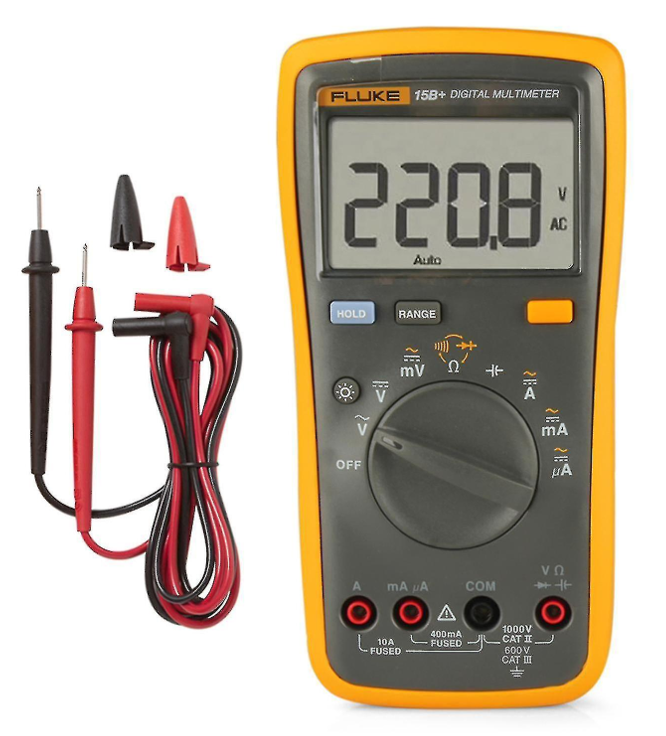
\includegraphics[width=0.6\linewidth]{img/multimeter.png}
        \caption{A multimeter}
        \label{fig:multimeter}
    \end{figure}

    \item \textbf{Measuring Current:}
    \begin{itemize}
        \item  Set the multimeter to the appropriate DC or AC current range based on the expected current you are measuring.
        \item Open the circuit at a convenient point and connect the multimeter in series with the break. The red lead typically goes to the positive side of the break.
        \item Read the displayed value on the multimeter. Caution: When measuring current, ensure the selected range is greater than the expected current to avoid damaging the meter.
    \end{itemize}

    \item \textbf{Measuring Resistance:}
    \begin{itemize}
        \item Set the multimeter to the resistance ($\Omega$) mode.
        \item Ensure the component being measured (resistor) is disconnected from any circuit.
        \item Touch the test leads to the terminals of the resistor.
        \item Read the displayed value on the multimeter. Note that some multimeter require holding the test leads for a stable reading.
    \end{itemize}

\end{enumerate}

\noindent \textbf{Part 2: Frequency Meter}

\begin{enumerate}
    \item Identify the input terminals on the frequency meter.
    \item Connect the frequency meter to the output of a signal generator using appropriate leads.

    \begin{figure}[H]
        \centering
        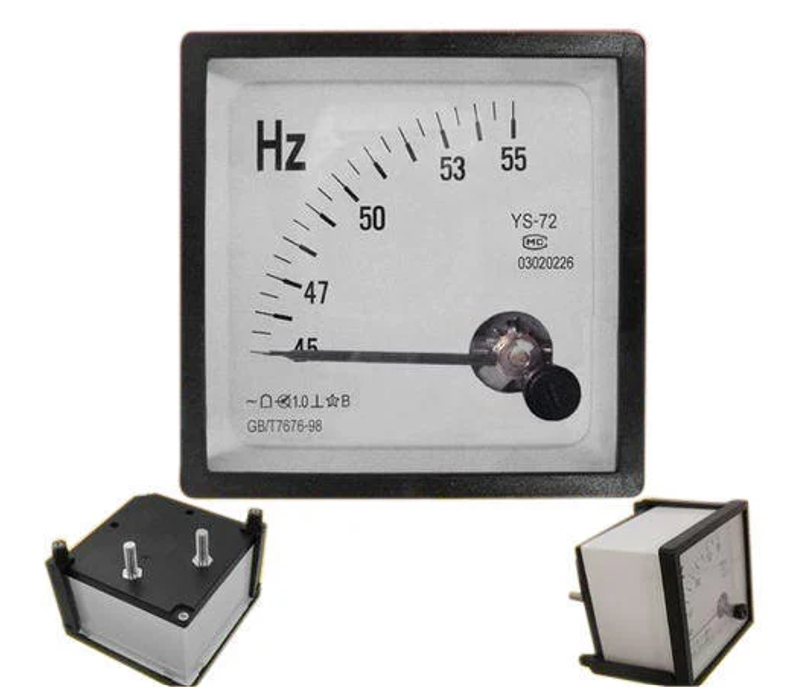
\includegraphics[width=0.5\linewidth]{img/freq_meter.png}
        \caption{Frequency Meter}
        \label{fig:enter-label}
    \end{figure}
    
    \item Set the signal generator to a specific frequency (e.g., 1 kHz, 10 kHz).
    
    \item Observe and record the reading displayed by the frequency meter. It should match the set frequency on the signal generator.
\end{enumerate}

\noindent \textbf{Part 3: Oscilloscope}
\begin{figure}[H]
    \centering
    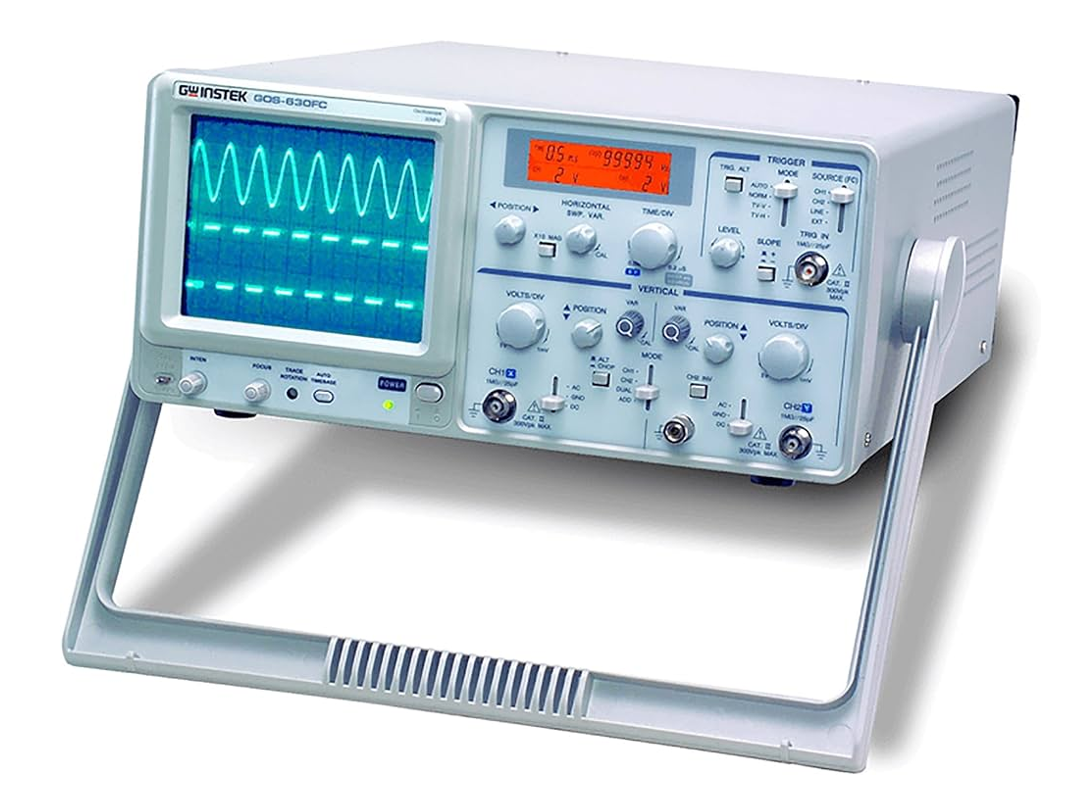
\includegraphics[width=0.7\linewidth]{img/oscilloscope.png}
    \caption{Oscilloscope}
    \label{fig:oscilloscope}
\end{figure}

\begin{enumerate}
    \item \textbf{Grounding:} Connect the ground clip of the oscilloscope probe to a common ground point in the circuit.

    \item Connect the oscilloscope probe tip to the point in the circuit where you want to observe the waveform.

    \item \textbf{Adjusting the Display:}
    
    \begin{itemize}
    
        \item Adjust the vertical scale (Volts/Div) to obtain a clear view of the waveform on the screen.

        \item Adjust the horizontal scale (Time/Div) to observe an appropriate number of cycles of the waveform.

        \item Use the trigger controls to achieve a stable display of the waveform.
        
    \end{itemize}

    \item \textbf{Signal Observation:}

    \begin{itemize}
    
        \item Set the signal generator to generate a sinusoidal waveform of a known frequency (e.g., 1 kHz).

        \item Observe the waveform displayed on the oscilloscope screen and measure the peak-to-peak voltage and frequency using the oscilloscope's graticule or cursors.

        \item Repeat the observation for different waveforms (e.g., square wave, triangular wave) generated by the signal generator.
        
    \end{itemize}

\color{red} A useful video on Oscilloscope: \href{https://www.youtube.com/watch?v=-qwzybAtvng}{Oscilloscope tutorial in Bangla by Rajib Sir BUET - YouTube}

\end{enumerate}

\noindent \textbf{Part 4: Signal Generator/Function Generator}

\begin{enumerate}
    \item Familiarize yourself with the controls of the signal generator. These typically include knobs for setting frequency, amplitude, waveform (sine, square, triangle), and output impedance.

    \item Set the desired frequency, amplitude, and waveform on the signal generator.

    \item Connect the output of the signal generator to the oscilloscope using appropriate leads.

    \item Observe the generated waveform on the oscilloscope screen and verify that it matches the settings on the signal generator.
    
    \begin{figure}[H]
        \centering
        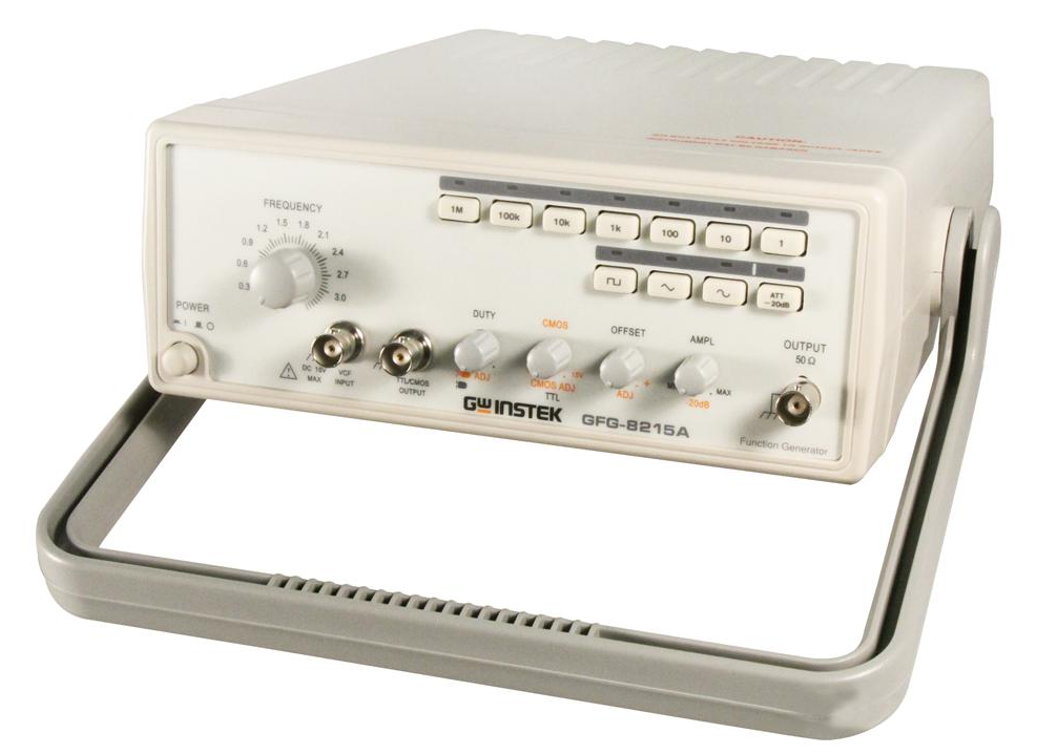
\includegraphics[width=0.75\linewidth]{img/signal_generator.png}
        \caption{Signal Generator}
        \label{fig:enter-label}
    \end{figure}

\end{enumerate}

\subsection*{Data and Calculations}

\begin{itemize}

    \item In a table, record the measurements obtained for voltage, current, resistance, and frequency using the multimeter and frequency meter.

    \item For the oscilloscope observations, sketch the waveforms observed for different settings on the signal generator and note down the measured peak-to-peak voltage and frequency.

\end{itemize}

\subsection*{Conclusion}
This lab experiment provided an introduction to the operation of basic electrical instruments. You should now be able to:

\begin{itemize}
    \item Identify and describe the functions of a multimeter, frequency meter, oscilloscope, and signal generator/function generator.
\end{itemize}

\newpage 
